\documentclass[11pt,a4paper]{article}
\usepackage[margin=22mm]{geometry}
\usepackage[T1]{fontenc}
\usepackage{lmodern,amsmath,amssymb,booktabs,longtable,array,enumitem,graphicx,xcolor,needspace}
\usepackage[hidelinks]{hyperref}
\usepackage{tikz}
\usetikzlibrary{arrows.meta,positioning,calc,circuits.logic.US}
\setlength{\parindent}{0pt}\setlength{\parskip}{0.5em}
\newcommand{\sol}{\paragraph{Solution.}}
\newcommand{\up}{\Uparrow}\newcommand{\dn}{\Downarrow}\newcommand{\any}{\Updownarrow}
\newcommand{\march}{\{\any(w0);\up(r0,w1);\up(r1,w0);\dn(r0,w1);\dn(r1,w0);\any(r0)\}}
\title{VLSI Testing: 2021 Final\\Reconstructed Questions and Independent Solutions}
\author{}\date{}
\hypersetup{pdftitle={VLSI Testing 2021 Final},pdfauthor={},pdfsubject={Reconstructed examination with independent solutions}}
\begin{document}\maketitle
This edition reconstructs the printed questions in three photographs. Handwritten answers and grading marks are not treated as an answer key. Editable functional redrawings, explicit fault models, and bit conventions accompany the independently derived solutions. A source-reading note identifies the BILBO control issue. The question weights total 100 points.

\section{Short questions (25 points)}
\begin{enumerate}[label=(\alph*)]
\item Why do March tests using only all-zero and all-one backgrounds fail to cover all coupling faults in word-oriented memories? (5 points)
\sol Bits of one word are written together. Solid backgrounds exercise equal-valued bit pairs without establishing both mixed states 01 and 10 inside a word. A coupling fault requiring an aggressor to be 0 while its victim is 1 may never be sensitized. Backgrounds such as 01010101, 00110011 and 00001111, and their complements for eight-bit words, distinguish bit positions and supply the missing relations. Inter-word coverage alone does not establish intra-word coverage.

\item How can the logic-BIST LFSR generate embedded deterministic patterns for random-pattern-resistant faults? (5 points)
\sol Derive test cubes by deterministic ATPG. For transition matrix $A$ over $\mathrm{GF}(2)$, the state after $k$ clocks is $A^ks$. Each specified cube bit supplies a linear equation in the seed $s$, including the scan decompressor or phase shifter's output transformation when present. Solve for a seed, load it, and run the prescribed shifts. Unspecified bits remain free variables. If one seed is insufficient, use multiple reseeds or another allowed polynomial. Store seeds and run lengths in the test controller or ROM. A short uncontrolled pseudorandom run does not guarantee application of a rare deterministic cube.

\item What should built-in self-diagnosis export? (5 points)
\sol Export the failing address or cell/bit position, expected and observed data or their XOR mask, and the failing March element/operation and background. Preserve failure order if it distinguishes candidate fault models. A final pass/fail bit cannot support localization and classification. A compressed failing-row/column map is suitable for redundancy allocation only if it retains the information that allocation needs.

\needspace{8\baselineskip}\item Distinguish concurrent and non-concurrent online BIST. (5 points)
\sol Concurrent online BIST checks the circuit while it performs normal operations, using the normal activity or associated check logic. Non-concurrent online BIST uses idle intervals or interrupts operation for an exclusive test window. Both occur during service life; only the concurrent form overlaps functional execution without taking over the tested resource.

\item A DRAM has a 32\,ms refresh period. Design a March test for stuck-at and retention faults. (5 points)
\sol Suppress refresh and other writes during each hold, and use
\[
 \any(w0);\ H_{\ge32\mathrm{ms}};\ \up(r0,w1);\
 H_{\ge32\mathrm{ms}};\ \up(r1).
\]
Start each global hold after the last write of the preceding phase. Every cell then holds each polarity for at least 32\,ms before verification. The two expected values expose both SAF polarities, while the holds expose loss of either stored polarity within the specified interval. Prevent refresh from concealing the defect and account for destructive reads. Coverage is for the stated single-cell retention model, not every possible history-, temperature- or timing-dependent DRAM fault.
\end{enumerate}

\section{Full scan and stuck-at tests (15 points)}
For the sequential circuit below, (a) make it scan testable, (b) derive tests for all combinational single stuck-at faults, and (c) describe their application. Each part is worth 5 points.

The photographed circuit has four flip-flops, two XNORs, an XOR, and a three-input NOR. Crossings without a connection do not join. Its equations are
\[
 a=\overline{X_2\oplus Q_1},\quad b=\overline{a\oplus Q_2},\quad c=b\oplus Q_3,
\qquad Y_1=\overline{X_1+c+Q_4},
\]
\[
 (D_1,D_2,D_3,D_4)=(b,Q_1,a,Q_3).
\]
\begin{figure}[ht]\centering
\begin{tikzpicture}[>=Latex,box/.style={draw,minimum width=16mm,minimum height=9mm},font=\small]
\node[box] (a) at (2,1.5) {XNOR};
\node[box] (b) at (5,1.5) {XNOR};
\node[box] (c) at (8,1.5) {XOR};
\node[box] (y) at (11,1.5) {NOR};
\draw[->] (0,1.5) node[left] {$X_2$}--(a.west);
\draw[->] (2,0) node[below] {$Q_1$}--(a.south);
\draw[->] (a)--node[above] {$a=D_3$}(b);
\draw[->] (5,0) node[below] {$Q_2$}--(b.south);
\draw[->] (b)--node[above] {$b=D_1$}(c);
\draw[->] (8,0) node[below] {$Q_3$}--(c.south);
\draw[->] (c)--node[above] {$c$}(y);
\draw[->] (11,3) node[above] {$X_1$}--(y.north);
\draw[->] (11,0) node[below] {$Q_4$}--(y.south);
\draw[->] (y)--(12.5,1.5) node[right] {$Y_1$};
\node at (5,-1) {$D_2=Q_1,\qquad D_4=Q_3$};
\end{tikzpicture}
\caption{Functional redraw of the logic exposed by full scan. The four state elements connect $D_i$ to $Q_i$ at a functional clock edge.}
\end{figure}
\sol (a) Replace every flip-flop with a scan flip-flop. Scan enable selects either its functional $D_i$ or the preceding scan bit. One valid chain is
\[
 \mathrm{SI}\to Q_1\to Q_2\to Q_3\to Q_4\to\mathrm{SO}.
\]
Full scan controls the four $Q_i$ and observes the four $D_i$, in addition to primary output $Y_1$.

(b) A complete test set is below. Inputs are $X_1X_2Q_1Q_2Q_3Q_4$; responses are $D_1D_2D_3D_4Y_1$.
\begin{center}\begin{tabular}{cc}\toprule Test&Response\\\midrule
000000&00101\\001011&11010\\010110&00010\\100000&00100\\000100&10100\\\bottomrule
\end{tabular}\end{center}
The public \texttt{tools/check\_recent\_exams.py} evaluates all 64 controllable input/state vectors. Its model contains both polarities on 14 named signal stems and 13 gate/buffer input branches: 54 single SAFs. The five vectors detect all 54, including fanout branches. Output buffers represent the separately observed $D_i$ branches. This claim excludes transistor, bridging, timing and scan-control faults.

At the NOR inputs $(X_1,c,Q_4)$, detecting input SA0s requires 100, 010 and 001, and SA1 detection requires 000. The checker enumerates the underlying six-bit vectors for these four classes and finds that no four-vector combination covers all 54 modeled faults. Thus five is also minimal for this explicit model.

(c) Assert scan enable and load the required state. For this chain order, shift $Q_4,Q_3,Q_2,Q_1$ into SI, in that temporal order. Deassert scan enable, apply $X_1X_2$, settle the logic and observe $Y_1$. Pulse the functional clock once to capture the $D_i$. Reassert scan enable and unload $D_4,D_3,D_2,D_1$, optionally overlapping unload with the next load. Compare the captured response, not the pre-capture state.

\section{March C-minus coverage (15 points)}
Explain why
\[
 \march
\]
covers stuck-at faults, transition faults, address-decoder faults, and state, inversion and idempotent coupling faults.

\sol The length is $10N$ for $N$ addressed bit cells. Every cell is written and read as both 0 and 1, detecting both SAF polarities. Rising and falling transitions are followed by verification reads before a legitimate overwrite can conceal the wrong value, detecting TFs.

The upward and downward sweeps establish both orders between different addresses. Under the usual single address-decoder fault model, a missing selection, unintended multiple selection, or address alias interferes with the contrasting old/new backgrounds and is exposed by a read.

For a coupling fault, let $a$ be its aggressor and $v$ its victim. CFin inverts $v$ when $a$ transitions; CFid forces $v$ on a transition; CFst forces $v$ for a specified state of $a$. Both aggressor transitions and both address orders ($a<v$ and $a>v$) are exercised. Complementary victim backgrounds ensure that a forcing effect disagrees with an expected read in one of the passes. Victim reads expose the corruption before restoration can mask it.

These are standard isolated static single-cell or unlinked two-cell assumptions. They do not include arbitrary linked, dynamic, retention or intra-word faults. The public checker independently confirms 28 explicit two-cell SAF/TF/CFin/CFid/CFst cases; that finite check supplements the reasoning and states its model.

\needspace{10\baselineskip}\section{Embedded-memory diagnosis flow (15 points)}
List the flow and the function of each step.
\sol
\begin{enumerate}
\item Select the fault models, diagnostic March operations and data backgrounds. Specify which observations distinguish candidate faults.
\item Apply patterns and compare reads with expected values. Record addresses, bit masks, operations and backgrounds.
\item Localize defective cells or lines and classify likely faults from the record. Apply additional diagnostic patterns if several candidates remain indistinguishable.
\item Construct a fault bitmap or equivalent compressed representation and perform redundancy analysis when spares are available.
\item Allocate legal spares, program or load the repair configuration, and retest the memory to check the allocation and spare resources.
\end{enumerate}
Detection, localization, classification, allocation and post-repair verification answer different questions. A failing memory may be repairable; a proposed repair is not verified until it passes a suitable retest.

\section{BILBO modes and polynomial (10 points)}
Three combinational blocks form a ring separated by four-bit BILBO registers. BILBO1 drives block~1 and BILBO2 collects its responses. (a) Determine their $B_1,B_2$ settings. (b) Find the polynomial. Each part is worth 5 points.

\begin{figure}[ht]\centering
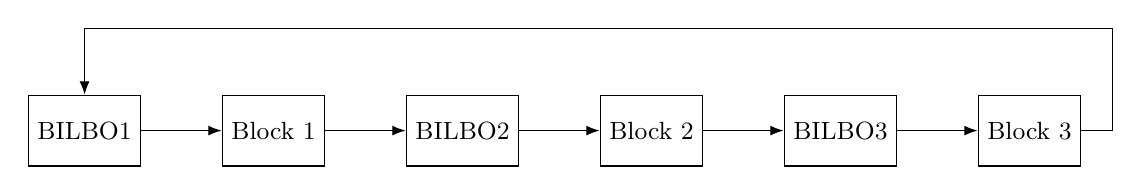
\begin{tikzpicture}[>=Latex,font=\small,r/.style={draw,minimum height=9mm,minimum width=13mm}]
\node[r] (r1) at (0,0) {BILBO1};
\node[r] (b1) at (2.4,0) {Block 1};
\node[r] (r2) at (4.8,0) {BILBO2};
\node[r] (b2) at (7.2,0) {Block 2};
\node[r] (r3) at (9.6,0) {BILBO3};
\node[r] (b3) at (12,0) {Block 3};
\draw[->](r1)--(b1);\draw[->](b1)--(r2);\draw[->](r2)--(b2);
\draw[->](b2)--(r3);\draw[->](r3)--(b3);
\draw[->](b3.east)--++(.4,0)|-(6,1.3)-|(r1.north);
\end{tikzpicture}
\caption{Redrawn BILBO ring. The repeated Block~3 label on the photograph's middle block is interpreted as a numbering typo.}
\end{figure}
\sol Read the gate implementation before assigning mode names. Its first-stage multiplexer has ScanIn on input 0 and feedback on input 1; the readable select line is $B_1$. Let $f=Q_2\oplus Q_3\oplus Q_4$ and $m=\mathrm{ScanIn}$ for $B_1=0$, otherwise $m=f$. The NOR/XOR network gives
\[
 D_1=(B_1Z_1)\oplus\overline{B_2+m},\qquad
 D_i=(B_1Z_i)\oplus\overline{B_2+Q_{i-1}}\quad(i=2,3,4).
\]
\begin{center}\begin{tabular}{ccl}\toprule $B_1$&$B_2$&Directly derived effect\\\midrule
0&0&Inverting serial shift from ScanIn\\
0&1&Clear all stages at the next clock\\
1&0&Feedback signature mode; PRPG when all $Z_i=0$\\
1&1&Parallel capture of $Z_1Z_2Z_3Z_4$\\\bottomrule
\end{tabular}\end{center}
BILBO2 uses 10 for response compaction. BILBO1 can use 10 as an autonomous pattern source only with its $Z_i$ held at zero and a suitable seed. Alternatively, apply external vectors through serial mode and account for scan inversion.

\textbf{Source-reading/feasibility note.} A supplied handwritten answer calls 00 a PRPG mode, but 00 selects ScanIn in the visible mux. An intended implementation with independently selectable feedback could support the familiar 00-generator/10-analyzer answer. The drawn ring does not by itself guarantee zero $Z_i$ at the generator, so autonomous operation requires that condition or a corrected control/mux design. This edition records the discrepancy rather than silently changing the circuit.

In feedback mode with $Z_i=0$,
\[
 Q'=(1\oplus Q_2\oplus Q_3\oplus Q_4,\,
 1\oplus Q_1,\,1\oplus Q_2,\,1\oplus Q_3).
\]
This is affine because of the NOR inversions. Its homogeneous transition matrix and characteristic polynomial are
\[
 A=\begin{pmatrix}0&1&1&1\\1&0&0&0\\0&1&0&0\\0&0&1&0\end{pmatrix},
 \qquad\det(xI-A)=x^4+x^2+x+1.
\]
The reciprocal delay/feedback-polynomial convention gives $x^4+x^3+x^2+1$. State-transition and reciprocal feedback conventions must be distinguished. Actual state/signature calculations must retain the affine constant vector; the polynomial alone is insufficient.

\section{IEEE 1149.1/1500 access (20 points)}
The system has two IEEE 1500-wrapped cores, a TAP with IR and bypass registers, Decoder~1 generating wrapper controls, Decoder~2 choosing routes, and a three-bit daisy-chain TAM. WIR1/2 are wrapper instruction registers and WBR1/2 are boundary registers. Answer (a) reset without a reset pin (3 points), (b) the source of controls $a,p$ (3), (c) decoding $q$ (4), and (d) serial and TAM external-test procedures (5 each).

\begin{figure}[ht]\centering
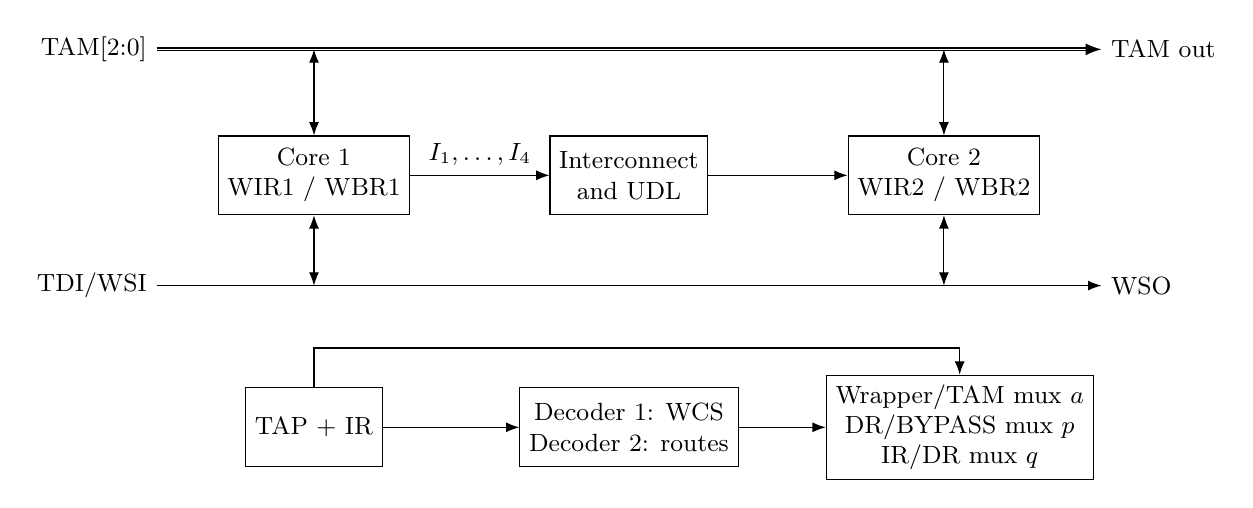
\begin{tikzpicture}[>=Latex,font=\small,box/.style={draw,align=center,minimum height=10mm}]
\node[box](c1)at(2,1.4){Core 1\\WIR1 / WBR1};
\node[box](u)at(6,1.4){Interconnect\\and UDL};
\node[box](c2)at(10,1.4){Core 2\\WIR2 / WBR2};
\draw[->](c1)--node[above]{$I_1,\ldots,I_4$}(u);\draw[->](u)--(c2);
\draw[->](0,0)node[left]{TDI/WSI}--(12,0)node[right]{WSO};
\draw[<->](2,0)--(c1);\draw[<->](10,0)--(c2);
\draw[->,double](0,3)node[left]{TAM[2:0]}--(12,3)node[right]{TAM out};
\draw[<->](c1)--(2,3);\draw[<->](c2)--(10,3);
\node[box](t)at(2,-1.8){TAP + IR};
\node[box](d)at(6,-1.8){Decoder 1: WCS\\Decoder 2: routes};
\node[box](o)at(10.2,-1.8){Wrapper/TAM mux $a$\\DR/BYPASS mux $p$\\IR/DR mux $q$};
\draw[->](t)--(d);\draw[->](d)--(o);
\draw[->](t.north)--++(0,.5)-|(o.north);
\end{tikzpicture}
\caption{Functional access-path redraw; boundary cells isolate core logic during an external interconnect test.}
\end{figure}
\sol (a) Hold TMS=1 for at least five TCK rising edges. Every TAP state then reaches Test-Logic-Reset. TMS=0 subsequently enters Run-Test/Idle. A dedicated TRST pin is optional; the question concerns the pinless reset path. The checker evaluates all 16 starting states.

(b) Both $a$ and $p$ come from Decoder~2's instruction-dependent route decoding. Mux $a$ selects the wrapper/TAM data source. Mux $p$ selects that result or the bypass-register output. Its lower input is connected to the bypass register, not the instruction register; the IR has a separate wire to the final output mux $q$.

(c) Mux $q$ selects the IR output in Shift-IR and the selected DR output in Shift-DR. It is decoded from TAP state. If input 1 is the IR and input 0 is the DR, a valid decode at the shifting states is $q=\mathrm{ShiftIR}$; reverse the polarity if the numbered mux inputs are reversed. TDO's data value is not meaningful in other states. The expression $\mathrm{ShiftIR}\lor\mathrm{ShiftDR}$ cannot select between the two paths, since it is one in both states. A TDO output-enable function, if implemented, is separate from the drawn data-selector $q$.

(d) Load the top-level \texttt{1500Test} instruction into the TAP IR and update it. Select WIR access, shift \texttt{ExTest} into both wrapper IRs, then update them. Load the farther WIR first in the serial chain; \texttt{1500Test} selects wrapper access and is not itself a wrapper instruction.

For the \emph{WSI--WSO route}, select WBR data access. Shift the launch vector into core~1 output boundary cells, update it to drive the interconnect/UDL, capture the response in core~2 input boundary cells, then unload through WSO/TDO. The symbolic selected path is
\[
 \mathrm{TDI/WSI}\to\mathrm{WBR1}\to\mathrm{WBR2}\to
 \mathrm{WSO}\to\mathrm{selected\ DR}\to\mathrm{TDO}.
\]
Repeat, overlapping unload with the next load when supported. Shift, update and capture are separate phases.

For the \emph{TAM route}, retain the \texttt{1500Test}/\texttt{ExTest} instructions but configure wrapper scan muxes and TAM outputs for the boundary-cell path. Distribute pattern portions through TAM to the launching wrapper cells, update, evaluate the UDL, capture at the receiving wrapper, and shift results to TAM out. Internal core scan chains should be isolated or bypassed: this tests interconnect, not core logic. WIR loading may still use the serial port even when test data use TAM.

The source's small selector labels are not all readable. These functional routes specify required connections without inventing binary settings for unreadable mux inputs.

\subsection*{TAP transition table}
This complete editable table is equivalent to the photographed state diagram.
\begin{center}\small
\begin{tabular}{lll}\toprule Current state&TMS=0&TMS=1\\\midrule
Test-Logic-Reset&Run-Test/Idle&Test-Logic-Reset\\
Run-Test/Idle&Run-Test/Idle&Select-DR\\
Select-DR&Capture-DR&Select-IR\\
Capture-DR&Shift-DR&Exit1-DR\\
Shift-DR&Shift-DR&Exit1-DR\\
Exit1-DR&Pause-DR&Update-DR\\
Pause-DR&Pause-DR&Exit2-DR\\
Exit2-DR&Shift-DR&Update-DR\\
Update-DR&Run-Test/Idle&Select-DR\\
Select-IR&Capture-IR&Test-Logic-Reset\\
Capture-IR&Shift-IR&Exit1-IR\\
Shift-IR&Shift-IR&Exit1-IR\\
Exit1-IR&Pause-IR&Update-IR\\
Pause-IR&Pause-IR&Exit2-IR\\
Exit2-IR&Shift-IR&Update-IR\\
Update-IR&Run-Test/Idle&Select-DR\\\bottomrule
\end{tabular}\end{center}
\end{document}
